\documentclass{article}

\usepackage{algorithm}
\usepackage{algpseudocode}
\usepackage{amsfonts}
\usepackage{amsmath}
\usepackage{caption}
\usepackage{dirtytalk}
\usepackage{hyperref}
\usepackage{mathtools}
\usepackage{multicol}
\usepackage{placeins}
\usepackage{siunitx}
\usepackage{subcaption}
\usepackage{tikz}
\usepackage{xypic}

\title{Spiral Ratchet \\[1ex] \large A Recursive Hash System}
\author{Brooklyn Zelenka \\ \href{https://fission.codes}{Fission Codes} \\ \href{mailto:brooklyn@fission.codes}{brooklyn@fission.codes} }
\date{\today}

\begin{document}
    \maketitle
   	\begin{abstract}\
   		This paper presents the spiral ratchet, a novel symmetric key derivation (KDF) chain that can be efficiently incremented by arbitrary intervals.
   	\end{abstract}

   	\section{Introduction}
   	
	Hash algorithms provide a way to generate deterministic but random-appearing data from an input that is impractical to reverse. Many applications iteratively hash a value (``ratcheting'') for pre-computation resistance, for backwards secrecy, one-time schemes (e.g. \href{https://datatracker.ietf.org/doc/html/rfc1760}{S/KEY}), deterministically generating unique names, key derivation functions (KDFs), and so on. We introduce the ``spiral ratchet'', a hierarchical iterative hashing system capable of efficiently making large leaps, while preserving backwards secrecy.

    \section{Motivation}
    
    The intersection of private data and location-independent access control in open distributed systems is only beginning to be explored. Trust minimized protocols are increasingly important, but admit to many unsolved problems, including how to secure changing data in an unknown and unstable topology.
    
    Functional persistence is a common strategy in distributed data. The security of history is very important in many applications, including group messaging, collaborative documents, time-series data, and even streams of data with micropayments. It is often impractical to perform a random key rotation for each update. Simple linear ratchets are often used in these situations, such as iteratively applying SHA3-256. More sophisticated ratchet mechanisms can be employed when the participants are fixed to a small group, such as \href{https://signal.org/docs/specifications/doubleratchet/doubleratchet.pdf}{Signal's Double Ratchet}.
    
    An increasing number of applications have an unstable topology of peers. They require zero-interaction key agreement for arbitrary keys in a sequence, the ability to share a single update (and no others), a range of updates, or history from a point in time onwards. As such, there is a need to keep the historical information of the KDF internal state secret as well.
    
    One approach for securing history is to use a simple ratchet function, iteratively hashing on each update to produce the next KDF state. This works well if the number of changes to synchronize is small, but $\mathcal{O}(n)$ ratchet generation steps is prohibitive as the difference grows. It allows a malicious participant to force others to perform the same amount of work.
    
    The spiral ratchet adds several properties. It synchronizes in sublinear time, supports efficient arbitrary access, its internal state is backwards secret, and its internal state does not leak metadata such as the number of updates. It is configurable to permit jumps of any size and granularity, and is weakly break-in resistant.
    
    \section{Numeral Intuition}
    
    The problem of how to quickly calculate the $n$th step of a ratchet in less than $n$ steps is structurally similar to how we efficiently represent large numbers. While not the only possible system, positional numeral systems are ubiquitous since they very elegantly and precisely express large numbers.
    
    \subsection{Unary Hashing}
   
    Unary is one of the simplest forms of representing numbers. This system is very concrete: the number of symbols is the number being represented. One example is tally marks, but the more computationally interesting are \href{https://en.wikipedia.org/wiki/Peano_axioms#Arithmetic}{Peano numbers}. These numerals are represented by a zero element 0, and successors $S$, such that the number 3 is represented $S(S(S(0)))$. This is very straightforward, but is neither space nor time efficient. 
    
	Peano numbers may expressed as functions via \href{https://en.wikipedia.org/wiki/Church_encoding}{Church-encoded}. Here, each successor is represented by function application. This model uses the constant identity function $\lambda{f}.\lambda{x}.x$ as ``zero'', and the application of a function to represent each successor, such that 3 is represented as $\lambda{f}.\lambda{x}.f(f(f x))$. Replacing the successor function with a hash function $h$, and an arbitrary initial value $I$ as its zero, one may represent unary counting structurally identically to Peano numbers. In this context, 3 is represented as the hash chain $h(h(h(I)))$.
	
    To avoid writing a large number of recursive applications by hand, let $h^n(I)$ be \emph{n} recursive applications of $h$ to $I$. By convention, this paper will use $I$, $J$, and $K$ as independent initial values.
    
    \subsection{Positional Hashing}
    
    A major advantage of positionality is the ability to express large jumps with minimal effort. In positional systems, such as the familiar binary, decimal, and hexadecimal, each position corresponds to some factor for the numeral at that position. While most systems have factors that are some exponent of a fixed base, there are many systems where there are no simple relationship between factors.
    
    \begin{figure}[h]
       	\centering
        $246_{16}$ = 2$\times{16^{2}}$ + 4$\times{16^{1}}$ + 6$\times{16^{0}}$ = $582_{10}$
     \caption{Componentized Hexadecimal}
    \end{figure}
    
    By analogy, multiple values can placed in a tuple and iteratively hashed to represent digits in a compound structure.
    
    \begin{figure}[h]
       	\begin{flalign}
       		h_{pos10}(0)   & \Rightarrow I \nonumber \\
       		h_{pos10}(11)  & \Rightarrow \langle h(J), h(I)\rangle \nonumber \\
       		h_{pos10}(582) & \Rightarrow \langle h^{5}(K), h^{8}(J), h^{2}(I) \rangle \nonumber 
       	\end{flalign}
       	
       	\caption{Compound Hash}
    \end{figure}
    
    Just as positional numerals combine multiple numbers to represent a single sum, a KDF can have multiple components that are combined to create a single symmetric key. Unlike a positional number system used in arithmetic, a KDF ``forgets'' its internal structure, combining elements and flattening its structure. There are many methods of combination, including further hashing; here we use binary $XOR$.
    
	\begin{figure}[h]
		\begin{flalign}
			h_{pos10, \oplus}(0)   & \Rightarrow I \nonumber \\
			h_{pos10, \oplus}(11)  & \Rightarrow h(J) \oplus h(I) \nonumber \\
			h_{pos10, \oplus}(582) & \Rightarrow h^{5}(K) \oplus h^{8}(J) \oplus h^{2}(I) \nonumber 
		\end{flalign}
	
		\caption{Compound Hash Key Derivation}
	\end{figure}
    
	While it is easier to reason about a consistent base, there are cases where the ability to skip by different intervals per level is useful. This paper will only consider the case where the base is consistent across all positional digits.
    
    \section{Bounding}
    
    Unlike number systems for arithmetic, the spiral ratchet has a fixed number of ``digits'' in its internal state. This limits the jumps to fixed intervals, with a maximum jump interval.  It would be possible to deterministically generate increasingly large digits as needed, but (as we will see later) this would leak data about the range that the count is currently in, which is undesirable (e.g. for securing updatable documents.)
    
    While ratcheting by arbitrary intervals is possible, the jump operation is not the same as adding arbitrary integers. Incrementing all but the lowest digit cascades down to the lower values, in effect ``zeroing'' them. Arbitrary jumps require a carry (Algorithm \ref{alg:jump}). This is structurally similar to \href{https://en.wikipedia.org/wiki/Skip_list}{skip lists} (Figure \ref{fig:skip-list}), but with each step pointing to a monotonically increasing value, rather than previous values. \\
 
	\begin{figure}[h]
		\centering
		
		$\xymatrix{
			  Nil
			& A \ar[l]
			& B \ar[l] , \ar@/^1pc/[ll]
			& C \ar[l]
			& D \ar[l] , \ar@/^1pc/[ll] , \ar@/_2pc/[llll]
			& E \ar[l]
			& F \ar[l] , \ar@/^1pc/[ll]
			& G \ar[l]
			& H \ar[l] , \ar@/^1pc/[ll] , \ar@/_2pc/[llll]
		}$
	
		\caption{Skip List}
		\label{fig:skip-list}
	\end{figure}

	\begin{figure}[h]
		\centering
		
		$\xymatrix{
		    \underset{000_{2}}{\left[ { \begin{array}{cc} L \\ M  \\ S \end{array} } \right]}
				\ar[r]^{+1}
				\ar@/_3pc/[rr]_{skip_{M}}
				\ar@/^7pc/[rrrr]^{skip_{L}}
    	 & \underset{001_{2}}{\left[ { \begin{array}{cc} L \\ M  \\ h(S) \end{array} } \right]}
	      		\ar[r]^{+1}
	      		\ar@/^4.75pc/[rrr]^{skip_{L}}
	     & \underset{010_{2}}{\left[ { \begin{array}{cc} L \\ h(M)  \\ S' \end{array} } \right]}
	      		\ar[r]^{+1}
	      		\ar@/_3pc/[rr]_{skip_{M}}
	      		\ar@/^3pc/[rr]^{skip_{L}}
    	 & \underset{011_{2}}{\left[ { \begin{array}{cc} L \\ h(M)  \\ h(S') \end{array} } \right]}
	      		\ar[r]^{+1}
	     & \underset{100_{2}}{\left[ { \begin{array}{cc} h(L) \\ M'  \\ S'' \end{array} } \right]}
		}$

		\caption{Simplified Compound Ratchet}
		\label{fig:compound-ratchet}
	\end{figure}

	Each digit is given a label and a maximum value for all but the largest, which acts as a linear spine. This treats the largest element as analogous to a unary digit, and the remaining elements are positional, bounded by their numerical base. The unary digit hides information about the range of numbers that the current internal state represents, which is called an ``epoch''.
	
	This is roughly analogous to moving along a spiral: one component returns to its initial value, but the other is always moving forward. The motion is predictable and roughly circular, but never crosses itself. Extending the metaphor further: following the spiral in single steps is smooth, but leaps are possible by crossing to adjacent rings.
	
	\begin{figure}[h]
		\centering
		
		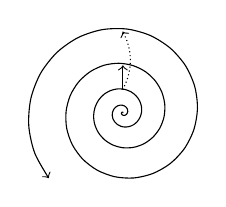
\begin{tikzpicture}
			\draw [->, domain=0:29, variable=\t, smooth, samples=100]
			plot ({\t r}: {0.0015 * \t * \t});
			\draw [->] (0, 0.3) -- (0, 0.6);
			\draw [->, style=densely dotted, rotate=-30] (-0.15, 0.250) arc (0:60:21pt);
		\end{tikzpicture}
		
		\caption{Spiral With Leaps}
		\label{spiral-metaphor}
	\end{figure}
	
	\section{Spiral Ratchet}
	
	The spiral ratchet is built from a unary digit $U$, a fixed number $n$ of positional digits, and their base $b$. The positional digits are bounded by the base, and so must track a natural number count. The unary digit explicitly does not track its count.
	
	\begin{figure}[h]
		\centering
		
		$\langle \langle Count_{0}, Value_{o} \rangle, \langle Count_{1}, Value_{1} \rangle \ldots \langle Count_{n-1}, Value_{n-1} \rangle, Unary \rangle_{b}$
		
		\caption{Spiral Ratchet State}
	\end{figure}

	Note that this is ordered as little-endian. The order of the state does not strictly matter, but it is convenient to associate the index of the state with the exponent for the base that the position represents.
	
	\subsection{Initialization}
	
	The base ratchet state is deterministically derived from a single initialization vector (IV). To prevent leaking the iteration count, all of the positional values are immediately incremented by a random value. This randomized origin is treated as the ratchet's initial value. Given the backwards secrecy constraint, only relative values may be used unless this initial value is known.
	
	Each positional value is generated from the \emph{binary complement of the preimage} of its larger neighbour, in a recursive cascade starting with the unary digit. This protects the information needed to derive the current state, and thus prevents leaking all of the values in that range.
		
	\begin{algorithm}
		\caption{Spiral Ratchet Initialization}
		\label{alg:setup}

		\begin{algorithmic}[1]
			\Require $(n, base, width) \in \mathbb{N}_{1}\times{\mathbb{N}_{1}\times{\mathbb{N}_{1}}}$
			\State $seed \gets random(0\ldots{2^{width}})$
			\State $state \gets \lbrace base = base, unary = hash(seed), pos = [] \rbrace$
			\For{$i \gets n - 1$ \textbf{to} $0$} \Comment{Descending to associate index with degree}
				\State $seed \gets hash(\sim{seed})$ \Comment{Secretly derive from the larger value}
				\State $\delta \gets random(0\ldots{base - 1})$
				\State $state[pos][i] \gets \{count = \delta, value = hash^{\delta + 1}(seed)\rbrace$
			\EndFor
			\\
			\Return{$state$}
		\end{algorithmic}
	\end{algorithm}

	The number of digits is a balance between granularity and jump control. If the number of digits is large, increment on the unary element or higher digits will have require multiple hash operations in each zero cascade.
	
	In practice, a 3-component (a unary spine and two positional digits) SHA3-256 spiral ratchet on base-256 has performed well. The maximum leap is $256^{2}$, which means that one can calculate the state for $i + 256^{3}$ in the same time as $i + 256$.

	\subsection{Basic Operations}
	
	Basic operations on the spiral ratchet follow from the basic rules set out during initialization. It can be incremented sequentially, or leap to the next ``zero'' of any digit. Any interval can be efficiently found by combining increments and leaps.
	
	\begin{figure}[h]
		\centering
		
		$\xymatrix{
			IV \ar[r]^<<<<<{inc} 
				& *+[F]{State_{0}}
					\ar[d]|\oplus
					\ar[r]^{inc}
					\ar@/^1.5pc/[rr]^{skip}
					\ar@{.>}@/^5pc/[rrrr]^{leap}
				& *+[F]{State_{1}}
					\ar[d]|\oplus
					\ar[r]^{inc}
					\ar@{.>}@/^3pc/[rrr]^{leap}
				& *+[F]{State_{2}} 
					\ar[d]|\oplus
					\ar[r]^{inc}
					\ar@/^1.5pc/[rr]^{skip}
				& *+[F]{State_{3}}
					\ar[d]|\oplus
					\ar[r]^{inc}
				& *+[F]{State_{4}}
					\ar[d]|\oplus
					\ar[r]^{inc}
				& \cdots
			\\
				& Key_{0}
				& Key_{1}
				& Key_{2}
				& Key_{3}
				& Key_{4}
		}$
		
		\caption{Spiral Ratchet Operations}
	\end{figure}

	Being a ratchet, it can never be ``unwound'' (there is no inverse or subtractive analogue). Access to earlier keys requires knowing an even earlier state, and moving forwards to the desired state from there. This is important for break-in resistance and backwards secrecy (e.g sharing a document from a point in time but no earlier).

	\subsubsection{Key Derivation}

	Generating output key material (OKM) from the ratchet state can be done in a myriad of ways. This paper will use the bitwise XOR function, as it is straightforward and efficient.

	\begin{algorithm}
		\caption{Generating a Key}
		\label{alg:toKey}

		\begin{algorithmic}[1]
			\Function{toKey}{ratchet}
				\State $sum \gets ratchet[unary]$
				\For{$digit \in ratchet[pos]$}
					\State $sum \gets acc \oplus digit[value]$
				\EndFor
				\State $sum$
			\EndFunction
		\end{algorithmic}
	\end{algorithm}

	\FloatBarrier
	
	\subsubsection{Incrementing}
	
	Just like positional numerals, when a digit reaches its maximum, the next larger digit is incremented, and all lower digits are zeroed out. The zero cascade works similarly for spiral ratchets, but never repeats a value (i.e. the \hyperref[{spiral-metaphor}]{spiral property}). Exactly like the initialization, each zero is derived from the preimage of the higher digit (Figure \ref{fig:zero-cascade}).
	
	\begin{figure}[h]
		\centering
		
		$\xymatrix{
		  h^{i-1}(U)
					\ar[r]^{h}
					\ar[dr]^{h \circ \sim}
				& h^{i}(U)
					\ar[rrrr]^{h}
					\ar[drrrr]^{h \circ \sim}
				&
				&
				&
				& h^{i + 1}(U)
					\ar[r]^{h}
				& \cdots
			\\    h(J_{-1})
					\ar[dr]^{h \circ \sim}
				& J_{0}
					\ar[rr]^{h}
					\ar[drr]^{h \circ \sim}
				&
				& h(J_{0})
					\ar[drr]^{h \circ \sim}
				&
				& J_{1}
					\ar[r]^{h}
				& \cdots
			\\  
				& I_{0}
					\ar[r]^{h}
				& h(I_{0})
				& I_{1}
					\ar[r]^{h}
				& h(I_{1})
				& I_{2}
					\ar[r]^{h}
				& \cdots
			\save
			"2,2" . "3,2" *[F.] \frm{}
			\restore
			\save
			"3,4" . "3,4" *[F.] \frm{}
			\restore
			\save
			"2,6" . "3,6" *[F.] \frm{}
			\restore
		}$
		
		\caption{Zero Cascade for a Binary Spiral Ratchet}
		\label{fig:zero-cascade}
	\end{figure}
	
	\FloatBarrier
	
	The special case of incrementing by one is the simplest way to demonstrate this (Algorithm \ref{alg:inc}). This functions by checking the lowest digit's counter, and if it's saturated, mark a carry and move to the next digit and recurse, bounded by the unary digit. Any carried digits are then re-zeroed by the preimage of their larger neighbour.
	
	\begin{algorithm}
		\caption{Incrementing a Spiral Ratchet}
		\label{alg:inc}

		\begin{algorithmic}[1]
			\Function{inc}{$ratchet$}
				\State $\{base, unary, pos\} \gets ratchet$
				\State $seed \gets unary$
				\State $counter \gets length(pos)$
				\\
				\For{$i \gets 0$ \textbf{to} $length(pos) - 1$}
					\State $\{count, value\} \gets pos[i]$
					\If{$count < base - 1$} \Comment{Position not saturated}
						\State $seed \gets value$
						\State $counter \gets i$
						\State $ratchet[pos][i] \gets \{ count = count + 1, value = hash(value)\}$
						\State \textbf{break}
					\EndIf
				\EndFor
				\\
				\If{$counter = length(pos)$} \Comment{All positional values were saturated}
					\State $ratchet[unary] \gets hash(unary)$
				\EndIf
				\\
				\If{$counter > 0$}
					\For{$j \gets counter - 1$ \textbf{to} $0$} \Comment{N.B. Descending}
						\State $seed' \gets pos[j][value]$
						\State $ratchet[pos][j][count] \gets \{count = 0, value = hash(\sim{seed})\}$
						\State $seed \gets seed'$
					\EndFor
				\EndIf
				\\
				\State $ratchet$
				\EndFunction
		\end{algorithmic}
	\end{algorithm}

	\subsubsection{Arbitrary Jumps}

	Jumps by an arbitrary interval require a little more calculation (Figure \ref{alg:jump}). The interval is componentized, and increments each digit in turn. Each digit has an upper bound, so any remainder saved for the final step, where any zeroed digits are incremented to match the final count.
	
	Each recursive zeroing is represented with a different value, both between digits and per-digit.

	\begin{algorithm}
		\caption{Spiral Ratchet Arbitrary Jump}
		\label{alg:jump}
		
		\begin{algorithmic}[1]
			\Function{jump}{$ratchet, amount$}
				\State $\{base, unary, pos\} \gets ratchet$
				\State $remaining \gets amount$
				\State $seed \gets unary$
				\State $carry \gets []$
				\State $n \gets length(pos)$
				\\
				\For{$i \gets 0$ \textbf{to} $n - 1$}
					\If{$remaining = 0$}
						\State \textbf{break}
					\EndIf
					\\
					\State $component_{i} \gets remaining\mod{base^{i}}$
					\State $remaining \gets remaining - component_{i}$
					\State $\delta_{i} \gets component\div{base^{i}}$
					\\
					\State $\{count, value\} \gets pos[i]$
					\State $headroom \gets base - count - 1$
					\\
					\If{$\delta_{i} > headroom$}
						\State $carry[i] \gets steps - headroom$
					\Else
						\State $ratchet[pos][i][count] \gets count + \delta_{i}$
						\If{$remaining = 0$}
							\State $seed \gets hash^{\delta_{i} - 	1}(value)$
							\State $ratchet[pos][i][value] \gets hash(seed)$
						\Else
							\State $carry[i] \gets 0$
						\EndIf
					\EndIf
				\EndFor
				\\
				\If{$remaining > 0$}
					\State $component_{u} \gets remaining \mod{base^{n}}$
					\State $\delta_{u} \gets component_{u}\div{base^{n}}$
					\State $ratchet[unary] \gets hash^{\delta_{u}}(unary)$
				\EndIf
				\\
				\For{$j \gets length(acc) - 1$ \textbf{to} $0$} \Comment{N.B. Descending}
					\State $seed \gets hash^{acc[j] - 1}(\sim{seed})$
					\State $ratchet[pos][j][value] \gets hash(seed)$
				\EndFor
				\\
				\State $ratchet$
			\EndFunction
		\end{algorithmic}
	\end{algorithm}

	\section{Security Considerations}
    
    \newpage
    
    \section{Acknowledgements}
    
    The spiral ratchet algorithm was developed at \href{https://fission.codes}{Fission Codes} to support work on the \href{https://github.com/fission-suite/webnative}{WebNative File System (WNFS)}. Many thanks to the Fission Codes team for providing the freedom to do this work.
    
    Thanks to \href{https://github.com/matheus23/}{Philipp Krüger} at Fission Codes for  feedback on the design, for writing the bulk of the \href{https://github.com/fission-suite/webnative/blob/e1eed4e750c668a6f54d9be701dc17e286b9eff4/src/fs/data/private/spiralratchet.ts}{TypeScript implementation}, and for his patience as various parts of the algorithm were tweaked.
    
    Thanks to \href{https://github.com/b5/}{Brendan O'Brien} at \href{https://qri.io/}{Qri} for the \href{https://github.com/qri-io/wnfs-go/blob/62915924c866f7106aecacccd14e57bd1b62850f/private/ratchet/ratchet.go}{Go implementation}, and for many discussions on the best way to explain the concept.
    
    Thanks to \href{https://github.com/dholms}{Daniel Holmgren} at \textbf{NOT YET PUBLIC} for his feedback on early versions of this algorithm.
    
    Thanks to \href{https://github.com/jbenet/}{Juan Benet} at \href{https://protocol.ai/}{Protocol Labs} for encouraging me to write a more full-fledged description of the spiral ratchet than what was available in the Fission Codes online documentation.
    
    The term “ratchet” for forward-secure key updating was introduced by Adam Langley in Pond [18]
    
    \bibliographystyle{plain}
    % FIXME FIXME FIXME
\end{document}
